%%%%%%%% ICML 2019 EXAMPLE LATEX SUBMISSION FILE %%%%%%%%%%%%%%%%%

\documentclass{article}

% Recommended, but optional, packages for figures and better typesetting:
\usepackage{microtype}
\usepackage{graphicx}
\usepackage{subfigure}
\usepackage{booktabs} % for professional tables
\usepackage{tabularx}

% hyperref makes hyperlinks in the resulting PDF.
% If your build breaks (sometimes temporarily if a hyperlink spans a page)
% please comment out the following usepackage line and replace
% \usepackage{icml2019} with \usepackage[nohyperref]{icml2019} above.
\usepackage{hyperref}

% Attempt to make hyperref and algorithmic work together better:
\newcommand{\theHalgorithm}{\arabic{algorithm}}

% Use the following line for the initial blind version submitted for review:
\usepackage{icml2019}
\newcommand{\bg}[1]{~{{[{\it \textcolor{red}{{\bf BG:} #1}}]}}}
\newcommand{\cs}[1]{~{{[{\it \textcolor{red}{{\bf CS:} #1}}]}}}
\newcommand{\ag}[1]{~{{[{\it \textcolor{red}{{\bf AG:} #1}}]}}}
% If accepted, instead use the following line for the camera-ready submission:
%\usepackage[accepted]{icml2019}

% The \icmltitle you define below is probably too long as aer.
% Therefore, a short form for the running title is supplied here:
\icmltitlerunning{Understanding the Black-box Structure of Epidemiology Simulators for Policy Decision Making}

\begin{document}

\twocolumn[
\icmltitle{Understanding the Black-box Structure of Epidemiology Simulators\\
			 for Policy Decision Making}

% It is OKAY to include author information, even for blind
% submissions: the style file will automatically remove it for you
% unless you've provided the [accepted] option to the icml2019
% package.

% List of affiliations: The first argument should be a (short)
% identifier you will use later to specify author affiliations
% Academic affiliations should list Department, University, City, Region, Country
% Industry affiliations should list Company, City, Region, Country

% You can specify symbols, otherwise they are numbered in order.
% Ideally, you should not use this facility. Affiliations will be numbered
% in order of appearance and this is the preferred way.
\icmlsetsymbol{equal}{*}

\begin{icmlauthorlist}
\icmlauthor{Aeiau Zzzz}{equal,to}
\icmlauthor{Bauiu C.~Yyyy}{equal,to,goo}
\icmlauthor{Cieua Vvvvv}{goo}
\icmlauthor{Iaesut Saoeu}{ed}
\icmlauthor{Fiuea Rrrr}{to}
\icmlauthor{Tateu H.~Yasehe}{ed,to,goo}
\icmlauthor{Aaoeu Iasoh}{goo}
\icmlauthor{Buiui Eueu}{ed}
\icmlauthor{Aeuia Zzzz}{ed}
\icmlauthor{Bieea C.~Yyyy}{to,goo}
\icmlauthor{Teoau Xxxx}{ed}
\icmlauthor{Eee Pppp}{ed}
\end{icmlauthorlist}

\icmlaffiliation{to}{Department of Computation, University of Torontoland, Torontoland, Canada}
\icmlaffiliation{goo}{Googol ShallowMind, New London, Michigan, USA}
\icmlaffiliation{ed}{School of Computation, University of Edenborrow, Edenborrow, United Kingdom}

\icmlcorrespondingauthor{Cieua Vvvvv}{c.vvvvv@googol.com}
\icmlcorrespondingauthor{Eee Pppp}{ep@eden.co.uk}

% You may provide any keywords that you
% find helpful for describing your paper; these are used to populate
% the "keywords" metadata in the PDF but will not be shown in the document
\icmlkeywords{Machine Learning, ICML}

\vskip 0.3in
]

% this must go after the closing bracket ] following \twocolumn[ ...

% This command actually creates the footnote in the first column
% listing the affiliations and the copyright notice.
% The command takes one argument, which is text to display at the start of the footnote.
% The \icmlEqualContribution command is standard text for equal contribution.
% Remove it (just {}) if you do not need this facility.

%\printAffiliationsAndNotice{}  % leave blank if no need to mention equal contribution
\printAffiliationsAndNotice{\icmlEqualContribution} % otherwise use the standard text.

\begin{abstract}

A goal of probabilistic programming is to couple simulators, with inference. This is 
because stochastic simulators are used prominently in many industrial settings,
do not require one to construct hand-crafted joint distributions as they implicitly 
define a joint distribution of the program and encode learnt structures 
directly. This makes simulators powerful tools and much of machine learning (ML) and 
Artificial Intelligence (AI)
can be seen as trying to emulate such simulators from a purely data-driven approach.
However, in the 
ML/AI setting, although we can often infer outcomes, we have little understanding about what 
in the data led to the outputted inferences. 
This makes it challenging to deploy ML/AI systems into the wild, especially in health-related and safety-critical domains, such
as epidemiology, as we lose \emph{interpretability}. 
In this work, we explain how to design ML/AI systems that combine
probabilistic programming systems (PPSs) and epidemiology simulators, to extract
fully interpretable structures, enabling policy makers 
and practitioners to make interpretable inferences. 
In particular, we demonstrate this for the Malaria disease in two commonly used simulators; EMOD and OpenMalaria.
\end{abstract}

\section{Introduction}
Ending the epidemics of AIDS, tuberculosis, malaria and other infectious diseases by 2030 is a key target within the Good Health \& Well-Being section of the UN Sustainable Development Goals \cite{refugees_2030_nodate}\cite{un_sustainable_2018}. 

Ending the epidemics of AIDS, tuberculosis, malaria and other infectious diseases by 2030 is a key target by the Good Health \& Well-Being section of the UN Sustainable Development Goals. 
Despite decades of substantial international efforts, malaria still annually kills about a quarter of a million children under the age of 5 in Africa alone.
Ending the epidemics of AIDS, tuberculosis, malaria and other infectious diseases by 2030 is a key target within the Good Health \& Well-Being section of the UN Sustainable Development Goals\cite{}. 

%maybe cut some of this paragraph out
% In contrast to AIDS, Malaria can be routinely cured thanks to the disposability of a variety of medical interventions. 
% Issues are further aggravated due to the increasing emergence of parasite resistance to multiple drugs, including artemisinin, or even insecticides. 
% Hence, despite decades of substantial international efforts, initial hopes of regional elimination or even global eradication have not been met.
%  So difficult is Malaria control that, even today, about a quarter of a million children under the age of 5 succumb to it every year in Africa alone. 

To reach the WHO’s target of reducing malaria incidence and mortality rates by at least 90\% by 2030, policymakers increasingly turn to evidence-based methods. 
However, the collection of large quantities of field data is often infeasible due to logistic, economic or political constraints, or outright impossible if novel methods are to be assessed a priori. 
Hence in silico simulation of malaria epidemiology plays an increasingly crucial role in evidence-based policymaking.

%Hence epidemiology simulators fine-tuned on real data play a crucial role in determining policy implications.
Even in the absence of political, economic and social constraints, Malaria epidemiology is governed by a complex set of drivers, few of which can be understood in isolation.
These include within-host dynamics, population-specific traits and even local geography.
Some progress in modeling specific components has been made, such as the parasite life-cycle, transmission vector dynamics and the inter-dependencies between infection rates and vicinity to open water. 
However, comprehensive modeling of all of these components in a regional context remains challenging, and is greatly impeded by the lack of available field data for regional calibration, hence the need for comprehensive simulators.
% Simulation complexity is further aggravated by considering feedback effects from a large arsenal of anti-malaria interventions, ranging from distribution of mosquito nets, indoor residual spraying and mass drug administration to age-specific vaccinations. 
Stochastic epidemiology simulators have already proven to be an invaluable tool to policymakers with policy implications that are often counterintuitive yet far-ranging. 
For example, it has been shown that mass vaccination may be largely ineffective in regions of large transmission rates, but may play a crucial role in areas of low transmittivity.


However, since many of these simulators are stochastic in nature and therefore act as black-boxes, understanding the structure of these complex simulators is challenging and poses several challenges for policy makers. 
Therefore, sophisticated tools are required that enable us to not only digest the results of the simulation, but provide pathways to perform complex inferences. 
To this end, we extend the work of \citep{baydin2018efficient} to enable multiple stochastic epidemiology simulators to be transformed into a probabilistic model that can be used as input to a probabilistic programming system, enabling trace paths to be extracted from the simulator on both a per human level and a population level, from which we can extract trace probabilities allowing policy makers to determine what actions have the biggest impact on the final output of the simulator and thus can shape policy decisions accordingly.
 We argue that our work is likely to have significant social impact on many livelihoods affected by Malaria and discuss opportunities for future research.

% Recent work by \citep{Baydin} introduces a fundamental paradigm change that allows to tackle the inverse problem directly. 
% Using a novel software tool named \textit{pyprob}, \citep{Baydin} extract program execution traces from state-of-the-art particle decay simulation engine SHERPA\cite{}.
%  Using latest techniques from universal probabilistic programming inference, the sampled execution traces are then used in order to characterise the posterior distribution of the simulator output. 
%  From these, regions in simulator input space can be associated with specified outcomes.

% SHERPA, however, is different from leading epidemiology simulators in that it does not simulate population dynamics, but instead models individual decays with different sampling strategies. Thus, the existing work of \cite{baydin2018efficient} must be extended to encapsulate these different strategies. 
%  In this paper, we for the first time demonstrate the applicability of \textit{pyprob}, and hence probabilistic programming inference, to population-based epidemiology simulators. 
%  In particular, we discuss how the leading malaria epidemiology simulators EMOD\cite{} and OpenMalaria\cite{} can be interfaced with \textit{pyprob}.
%   We argue that our work is likely to have significant social impact on many livelihoods affected by Malaria and discuss opportunities for future research.

% maybe talk about this framework enables a pathway to inference etc..

% All of the above limitations require contemporary malaria epidemiology simulators to employ stochastic modeling techniques, which negotiate data scarcity and model uncertainty through the use of appropriate prior distributions that can be tuned even from small samples of field data. The population dynamics of groups of typically several thousand hosts are then initialised by sampling from the initial distributions, using initial random seeds. Forward simulation then proceeds by rolling out population dynamics over time. Simulation outcomes of cherry-picked scenarios and interventions of interest are then compared to suitably designed control runs.

% This is great, if we had inference implemented right now.
% However valuable forward simulations of epidemiology scenarios are, the holy grail of goal-driven policymaking ultimately lies in solving the inverse problem: Given a desired outcome and regional context, identify the series of interventions that will best reach the desired target after a given amount of time. Due to computational constraints, even an approximate search over the whole simulator input space usually proves intractable. An experience-guided search over the simulation output of a small set of manually-designed scenarios of interest therefore long seemed the only feasible way of investigating implications of policy interventions.


% , and, above all, the lack of available field data for calibration, 

% parasite life-cycle, transmission vectors, population dynamics and even local geographic circumstances, with policy measures ranging from distribution of mosquito nets to experimental vaccines, requires such simulators to be stochastic. Simulation outcomes thus need to be evaluated on a population of subjects.

% <Section about prob prog inference, with reference to SHERPA>

%- issues of public health are complex and 

%To do. 
%
%\begin{itemize}
%
%\item Outline the objectives
%\item State the importance of interpretability in the inference of the simulator
%\item Our system enables one to understand and interpret the most common paths in a program (simulation).
%\item In highlighting this a practitioner can then go back to the field and explore that parameter/s in more depth.
%\item This facilitates understanding and the construction of more detailed models and data collection strategies
%
%
%\end{itemize}
%
%% taken from Toms thesis. 
%
%Stochastic simulators are common across a number of domains, statistical physics~\cite{landau_binder_2014}, financial modeling~\cite{jackel2002monte},
%weather prediction~\cite{evensen1994sequential}, epidemiology~\cite{smith2008towards} and many others. 
%An advantage of using stochastic simulators is that they provide a level of interpretability not found in modern deep learning settings, as they directly incorporate model structure from carefully reasoned observations and experiments.  
%Probabilistic programming systems~(PPSs) are purpose built systems for making inferences and probabilistic 
%modeling accessible. 
%In particular, PPSs allow probabilistic models to be represented in the form of a generative model through the
%probabilistic programming language~(PPL), which enables one to write statements that enable conditioning on data~\cite{gordon2014probabilistic,Goodman08church:a}. 
%Thus, it seems only natural to connect simulators with PPSs, as simulators explicitly define a generative model, in the language in which they are written, and the nature of the PPSs enables us to perform inference in these simulators, by conditioning on observations, which are fed in as input to the simulators. 
%In doing this we can infer things about stochastic input parameters and other variables sampled during the program's forward execution, whilst also providing full interpretability in the inference results, which is absolutely necessary in safety-critical domains.
%By exploiting the tools that we develop in this paper, one is able to connect epidemiology simulators with \texttt{Pyprob}~\cite{le-2016-inference} to extract fully interpretable posterior structures allowing practitioners to interpret which input parameters have the largest affect on the epidemic, in our case malaria. Over five-hundred-thousand people die from malaria each year, mostly children under five years of age, with 90 per cent of malaria cases occurring in Sub-Saharan Africa. An estimated 100-300 million people suffer from malaria each year~\cite{world2016world}. 
%Thus, by understanding the prominence of input parameters to epidemiology simulators, guides decision making processes relating to effective treatment and prevention strategies. 
%\label{sec:related}


\section{Epidemiology Simulators and Probabilistic Programming}
\label{sec:background}



\subsection{Probabilistic Programming}
Probabilistic programming~\cite{gordon2014probabilistic,staton2016semantics,kozen1979semantics} is the coming together of multiple disciplines; computer science, statistics and machine learning. 
It attempts to unify the three fields by creating automated frameworks in which one can easily extrapolate their observed data and perform sophisticated statistical analysis with advance inference procedures such as 
Markov Chain Monte Carlo (MCMC), Variational Inference~(VI) and Deep Neural Networks~(DNN) in an accessible way, i.e. without the need of expert knowledge in implementing and using such procedures.
Users can then exploit these algorithms on an array of models
within the probabilistic programming language~(PPL), using the language itself to create models that represent complicated distribution objects. 
PPLs typically extend existing programming languages such as python, c++, go and so forth, which means that users do not have to learn
a completely new set of operating semantics.  
Our PPL PyProb~\cite{le-2016-inference,baydin2018efficient} belongs to the family of universal PPLs 
that allow the expression of unrestricted probability models in a Turing complete fashion~\cite{wood2014new,goodman2012church,landau_binder_2014,siddharth2017learning,bingham2019pyro}.

\subsection{Stochastic Simulators}

Simulators encode several years, if not decades, of research and development and so by their very nature are structurally complicated. Within the context of epidemiology simulators we can model treatment, infection and prevention cycle under a variety of different environmental conditions, enabling predictions to be made given a series of field observations \bg{Make sure that I do not state they can already do what PP can do, i.e. the ability to update and infer the input parameters continually conditioned on new observations.}.
However, since the development happens over several decades, usually without comprehensive documentation, understanding a code base written with legacy libraries and software is incredibly difficult and an almost impossible task for a non-expert, or expert who has not had access to the previous years of development. 
Our method of hijacking simulators builds on the work of~\cite{baydin2018efficient} and extends the framework to encapsulate a more diverse range of simulators. Our framework provides a simple solution and makes it easy to transform arbitrary stochastic simulators into probabilistic programs, regardless of the complexity of the simulator and the language that the simulator is written in\footnote{The framework currently supports 9 popular languages, but there is nothing to stop this being extended to any language of interest.}. 
In addition to this, we can understand the structure of programs in simulators for both decoding \emph{black-box structures} and for posterior inference. This enables two things. 
1) It enables software developers and policy making to understand complicated code bases and dissect outputs of simulators.
 2) It provides interpretable inference results that provide policy makers with predictions that are truly interpretable, in the sense that the end-user of the inference results understands what physical events led to the inference outcome. 
 This is critical in several domains, especially in epidemiology. 
 We provide examples of former in next Section~\ref{sec:casestudy} and discuss the latter in ~\bg{Link to conclusion / future work}.


 \subsubsection*{Epidemiology Simulators}
 \paragraph*{OpenMalaria} Write a small paragraph on openmalaria, 
 What is openmalaria? Open Malaria is an open-source simulator funded by the Gates Foundation to model different  aspects of the malaria prevention and treatment cycle for varying population dynamics.
 Models in OpenMalaria are specified via a scenario file, in the form of an XML document, which specifies the specifics of a particular treatment, or prevention strategy, climatic factors, the demographics of the population and so forth. In addition to this, field observations can be encoded inside of, or externally to the scenario file. 
The scenario file encodes all input and output parameters, some of which we wish to simulate to try and infer, others remain fixed. 

 \paragraph{EMOD} Do the same for EMOD as OM

\section{Case Study}
\label{sec:casestudy}
\subsection{Connecting a Epidemiology Simulators to a Probabilistic Programming System}

In order to hijack the stochastic simulator we are only required to override the location of the stochastic primitives, i.e. the operations that generate the stochasticity and randomness within the simulator. 
We will walk through how this is done for EMOD and OpenMalaria, you will see that it is procedurally identical.
However, given the sheer number of simulators it maybe slightly different procedurally. 
To our knowledge it shouldn't be, but we have not been able view of all stochastic simulators we cannot make this guarantee with certainty. 
The first step is to build a containerized environment, such as Docker~\cite{merkel2014docker} and Singularity~\cite{kurtzer2017singularity}, which enables the simulators to be run on any device, independent of different hardware architectures, removing the requirement for hardware specific machines. 
This greatly improves the scope of applicability of our system, as this environment only has to be built once, which then enables the simulator to be run simultaneously on machines of different architectures machine. 
The second step requires one to override the stochastic primitives, which requires re-writing aspects of the sampling procedures inside the simulator. 
This requires zero domain-expertise and only requires one to find where the sampling calls are originated, this can be done with any basic editor search function.
 Such information is typically saved in $\texttt{RANDOM.<filetype>}$.  We now demonstrate this for a normal primitive. 
\bg{Add code snippet here showing original code then modified code}
The third step is creating the protocols, which enable communication between the simulator and probabilistic programming system. 
For this we extend the existing bringing framework introduced in~\cite{baydin2018efficient}, which is comprised of the Probabilistic Programming eXecution~(PPX) protocols and a light-weight c++ interface, however this light-weight interface is dependent on whatever the file type of the $\texttt{RANDOM.<filetype>}$ file is.
In doing this we enable a larger class of sampling procedures to be overridden. The PPX protocols in particular take advantage of flat buffer protocols \bg{add cite to google fb}, which require a flatbuffers script to be specified, see here for an example of a flat buffers script \bg{reference PPX github page}. Once this is specified the flat buffers script is compiled and automatically constructs the message passing framework between the simulator and the probabilistic programming system. 
The next steps requires modifying the $\texttt{main}$ function in $\texttt{main.cpp}$, \bg{add more on this later}
The final step is to create a light-weight interface. As both the EMOD and OpenMalaria are solely based on c++ we can extend an existing interface called pyprob\_cpp\footnote{Add github link here} to account for the additional sampling procedures.
Once these steps are complete, the containerized environment will now contain everything required to pass models through to the simulators, encode the simulator into a probabilistic program, which can then be evaluated in the probabilistic programming system. We provide examples of this output in Figure~\ref{fig:plotewan}. 

% \subsection{Extending Probabilistic Programming Protocols}

\begin{figure*}[h!]
	\centering
	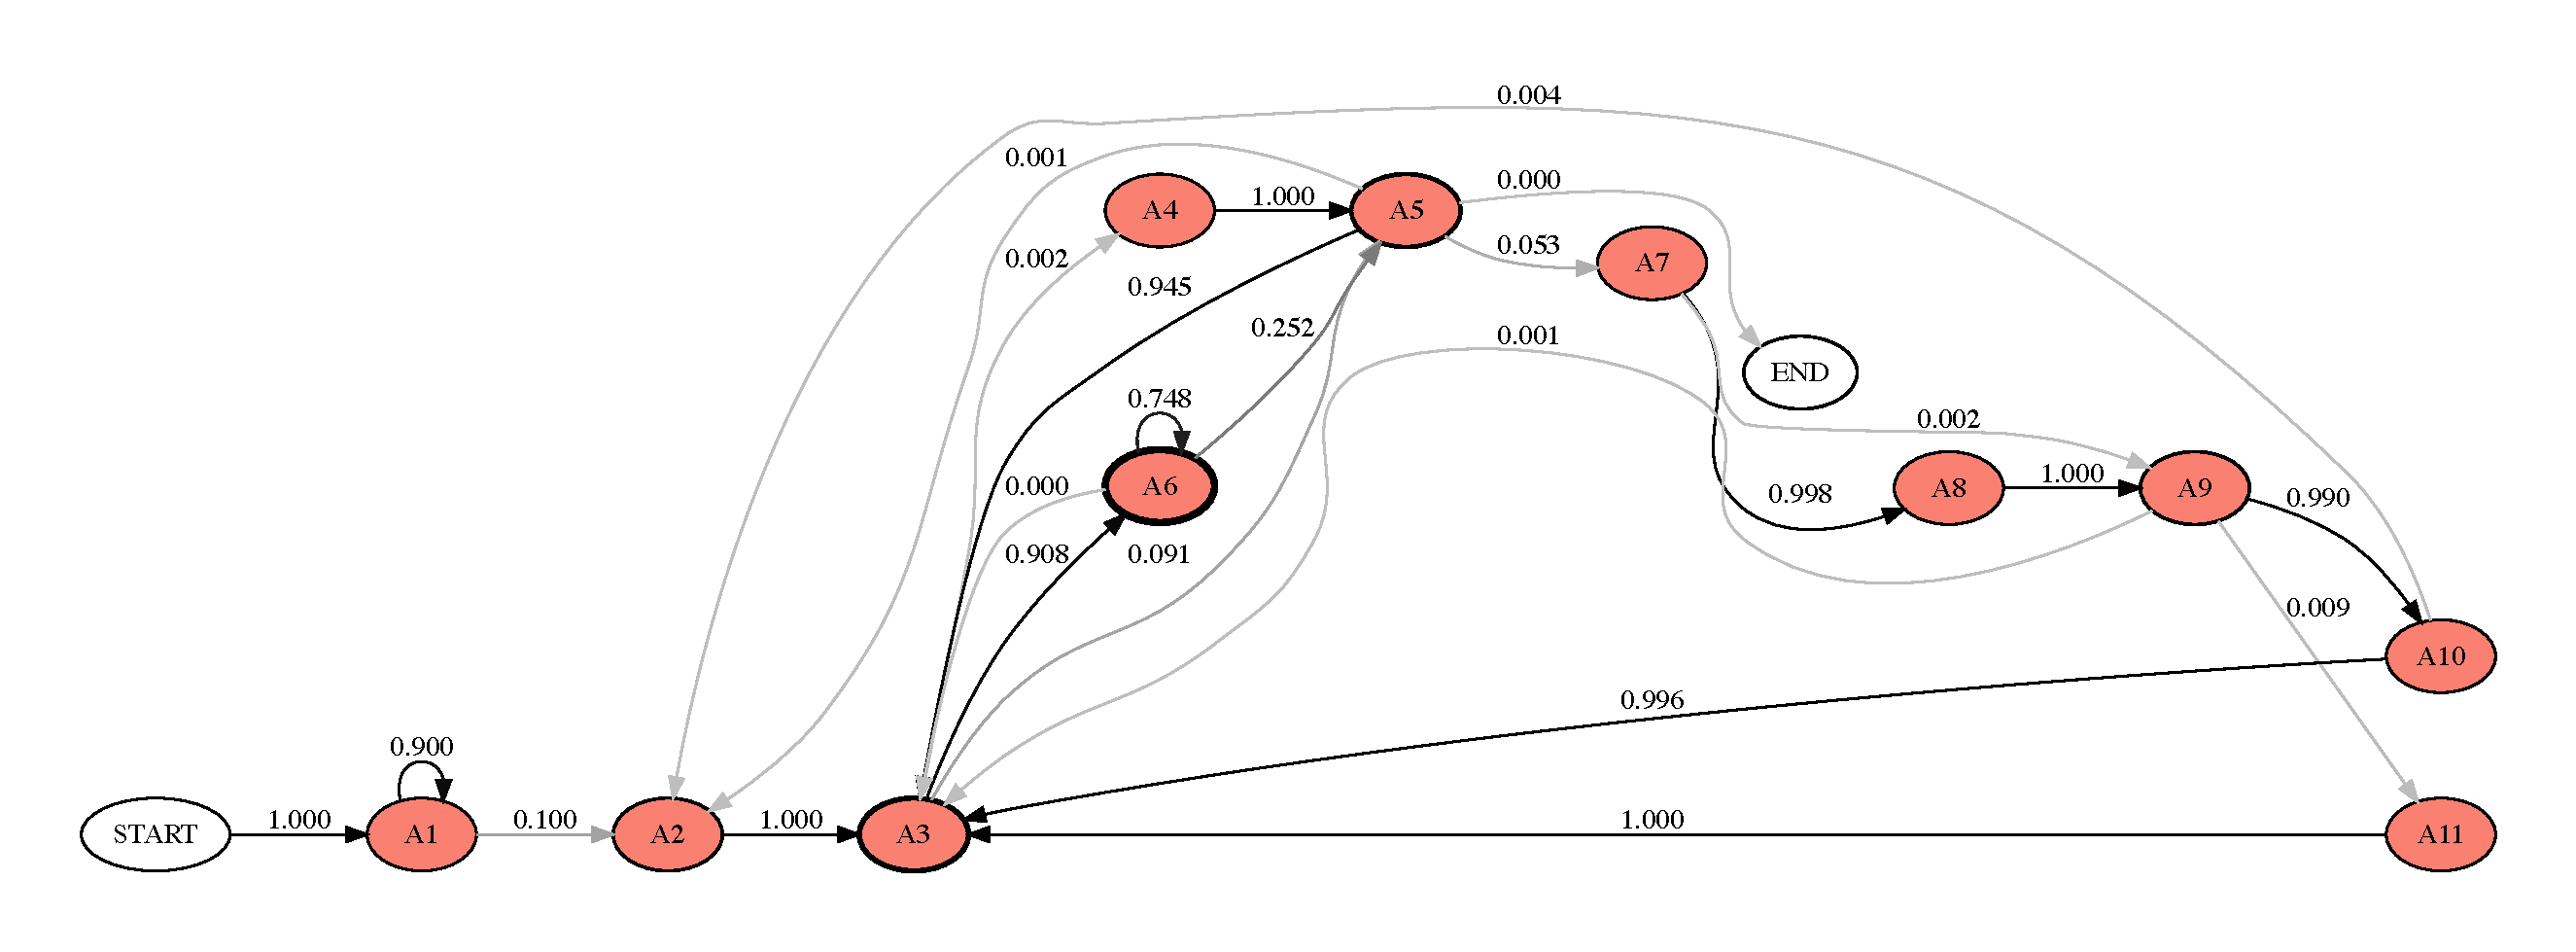
\includegraphics[width=\textwidth]{../plots/ewan_25_pop_10.pdf}
	\centering
	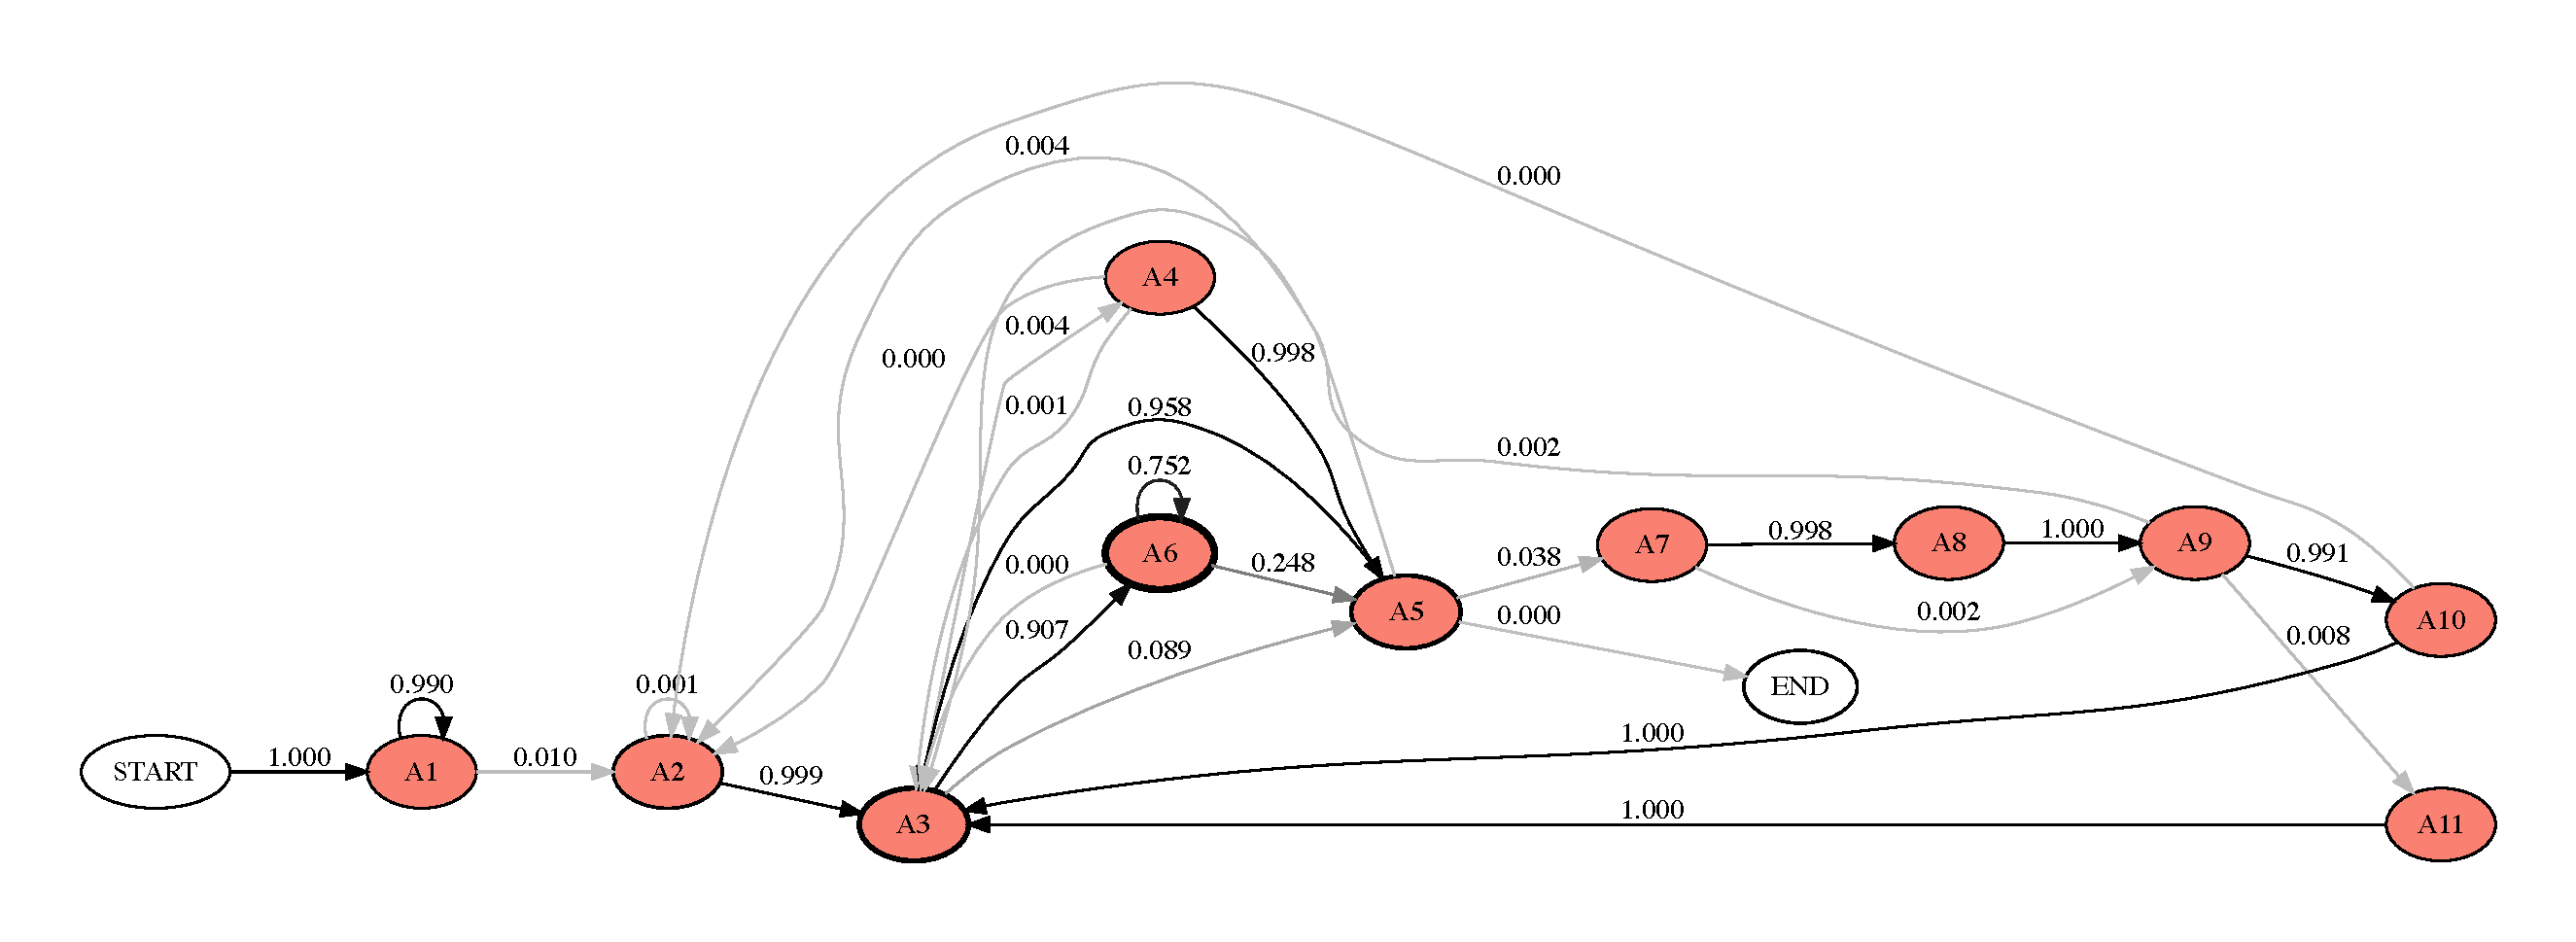
\includegraphics[width=\textwidth]{../plots/ewan_25_pop_100.pdf}
	\caption{Add something. Population 100}
	\label{fig:plotewan}
\end{figure*}
TODO

% Please add the following required packages to your document preamble:
% \usepackage{booktabs}
% Please add the following required packages to your document preamble:
% \usepackage{booktabs}
% \usepackage{graphicx}
% Please add the following required packages to your document preamble:
% \usepackage{graphicx}
  \begin{table*}[h!]
  \footnotesize
  \setlength{\tabcolsep}{1mm}
  \caption{Addresses }
  \label{table:addresses}
  \def\arraystretch{1.25}
  % \setlength{\tabcolsep}{1mm}
  \begin{tabularx}{\textwidth}{@{}lX@{}} 
    \toprule
    Address ID & Full address \\
    \midrule
  A1 & [forward()+0x204; OM::Simulator::start(scnXml::Monitoring const)+0x28a;

  OM::Population::createInitialHumans()+0x94;
  
  OM::Population::newHuman(OM::SimTime)+0x5c;

  OM::Host::Human::Human(OM::SimTime)+0x12b;

  OM::WithinHost::WHInterface::createWithinHostModel(double)+0x99;

  OM::WithinHost::DescriptiveWithinHostModel::DescriptiveWithinHostModel(double)+0x3a;

  OM::WithinHost::WHFalciparum::WHFalciparum(double)+0xe6;

  OM::util::random::gauss(double, double)+0xb4]\_\_Normal\\

   $\vdots$ & $\vdots$ \\
  A5 & [forward()+0x204; OM::Simulator::start(scnXml::Monitoring const\&)+0x468;

   OM::Population::update1(OM::SimTime)+0xff;

    OM::Host::Human::update(bool)+0x2bc;

    OM::Clinical::ClinicalModel::update(OM::Host::Human\&, double, bool)+0x96;

    OM::Host::NeonatalMortality::eventNeonatalMortality()+0x9;

    OM::util::random::uniform\_01()+0xc0]\_\_Uniform\\

%   A6 & [forward()+0x204; OM::Simulator::start(scnXml::Monitoring const\&)+0x468;

%    OM::Population::update1(OM::SimTime)+0xff;

%    OM::Host::Human::update(bool)+0x280;

%    OM::WithinHost::DescriptiveWithinHostModel::update(int, std::vector \textgreater{}\&, double, double)+0x3a2;

%    OM::WithinHost::DescriptiveInfection::determineDensities(double, double, double, double\&, double, double)+0x303;

%    OM::util::random::uniform\_01()+0xc0]\_\_Uniform\\
%    A7 & [forward()+0x204; OM::Simulator::start(scnXml::Monitoring const\&)+0x468;
%    ı
% 	OM::Population::update1(OM::SimTime)+0xff;

% 	OM::Host::Human::update(bool)+0x2bc;

% 	OM::Clinical::ClinicalModel::update(OM::Host::Human\&, double, bool)+0xe8;

% 	OM::Clinical::CM5DayCommon::doClinicalUpdate(OM::Host::Human\&, double)+0x67;

% 	OM::WithinHost::WHFalciparum::determineMorbidity(OM::Host::Human\&, double, bool)+0x73;
% ı
% 	OM::WithinHost::Pathogenesis::PathogenesisModel::determineState(OM::Host::Human\&, double, double, double, bool)+0x143;

% 	OM::util::random::bernoulli(double)+0x47;

% 	OM::util::random::uniform\_01()+0xc0]\_\_Uniform\\
% 	A8 & [forward()+0x204; OM::Simulator::start(scnXml::Monitoring const\&)+0x468;

% 	OM::Population::update1(OM::SimTime)+0xff; OM::Host::Human::update(bool)+0x2bc;

% 	OM::Clinical::ClinicalModel::update(OM::Host::Human\&, double, bool)+0xe8;

% 	OM::Clinical::CM5DayCommon::doClinicalUpdate(OM::Host::Human\&, double)+0x67;

% 	OM::WithinHost::WHFalciparum::determineMorbidity(OM::Host::Human\&, double, bool)+0x73;

% 	OM::WithinHost::Pathogenesis::PathogenesisModel::determineState(OM::Host::Human\&, double, double, double, bool)+0x162;

	% OM::util::random::bernoulli(double)+0x47;

% 	OM::util::random::uniform\_01()+0xc0]\_\_Uniform\\
% A9 & [forward()+0x204; OM::Simulator::start(scnXml::Monitoring const\&)+0x468;
%  OM::Population::update1(OM::SimTime)+0xff; OM::Host::Human::update(bool)+0x2bc;

%  OM::Clinical::ClinicalModel::update(OM::Host::Human\&, double, bool)+0xe8;

%   OM::Clinical::CM5DayCommon::doClinicalUpdate(OM::Host::Human\&, double)+0x67;

%   OM::WithinHost::WHFalciparum::determineMorbidity(OM::Host::Human\&, double, bool)+0x73;

%   OM::WithinHost::Pathogenesis::PathogenesisModel::determineState(OM::Host::Human\&, double, double, double, bool)+0x1c7;

%   OM::util::random::bernoulli(double)+0x47; OM::util::random::uniform\_01()+0xc0]\_\_Uniform\\
 $\vdots$ & $\vdots$ \\

% A11 & [forward()+0x204; OM::Simulator::start(scnXml::Monitoring const\&)+0x468;

% OM::Population::update1(OM::SimTime)+0xff; OM::Host::Human::update(bool)+0x2bc;

% OM::Clinical::ClinicalModel::update(OM::Host::Human\&, double, bool)+0xe8;

% OM::Clinical::CM5DayCommon::doClinicalUpdate(OM::Host::Human\&, double)+0xad;

% OM::Clinical::CM5DayCommon::severeMalaria(OM::Host::Human\&, OM::Clinical::Episode::State, double, int\&)+0x4b1;

% OM::util::random::uniform\_01()+0xc0]\_\_Uniform\\

\bottomrule
  \end{tabularx}
  \end{table*}


\bibliographystyle{icml2019}
\bibliography{malaria,refs}


\end{document}


% This document was modified from the file originally made available by
% Pat Langley and Andrea Danyluk for ICML-2K. This version was created
% by Iain Murray in 2018, and modified by Alexandre Bouchard in
% 2019. Previous contributors include Dan Roy, Lise Getoor and Tobias
% Scheffer, which was slightly modified from the 2010 version by
% Thorsten Joachims & Johannes Fuernkranz, slightly modified from the
% 2009 version by Kiri Wagstaff and Sam Roweis's 2008 version, which is
% slightly modified from Prasad Tadepalli's 2007 version which is a
% lightly changed version of the previous year's version by Andrew
% Moore, which was in turn edited from those of Kristian Kersting and
% Codrina Lauth. Alex Smola contributed to the algorithmic style files.
